\documentclass{f4_beamer}

\title{"Earned value" Methode aus dem klassischen Projektmanagement}
%\subtitle{Untertitel}
\author{Nick Marlon Grunert}
\date{\today}

\begin{document}

\section{Einführung}

\begin{frame}{Einführung}
    \begin{itemize}
        \item Einführungstext
        \item Noch mehr
        \item bitte funktioniere
    \end{itemize}
\end{frame}

%\section{simpleSlides}

% [fragile] is needed for the \verb|...| command to work. It is magic and show
% it up if you want to know how it works.
% NOTE: keep in mind that the use of fragile the build time increases
\begin{frame}[fragile]
    Change the labels using \verb|\item[label text]| in an
    \texttt{itemize} environment

    \begin{itemize}
        \item This is my first point
        \item Another point I want to make
        \item[!] A point to exclaim something!
        \item[$\blacksquare$] Make the point fair and square.
        \item[NOTE] This entry has no bullet
        \item[] A blank label?
    \end{itemize}
\end{frame}

\begin{frame}[fragile]
    Change the labels using \verb|\item[label text]| in an
    \texttt{enumerate} environment
    \begin{enumerate}
        \item This is my first point
        \item Another point I want to make
        \item[!] A point to exclaim something!
        \item[$\blacksquare$] Make the point fair and square.
        \item[NOTE] This entry has no bullet
        \item[] A blank label?
    \end{enumerate}
\end{frame}
%\section{pictureSlides}

\begin{frame}
    \begin{figure}[htp]
        \centering
        
\includegraphics[width=.8\textwidth, keepaspectratio]{%
            % image has to be relative to the actual f4_beamer.tex because
            % this file is being included there. Hence, if the image is relative
            % to this current directory it will not work.
            pictureSlides/test-image.jpg
        }
        \caption{%
            https://www.pexels.com/de-de/foto/natur-dunkel-wald-baume-6992/
        }
    \end{figure}
\end{frame}

\begin{frame}
    \begin{figure}[!tbp]
        \centering
        % https://www.namsu.de/Extra/befehle/Minipage.html
        \begin{minipage}{0.5\textwidth}
            
\includegraphics[width=\textwidth]{pictureSlides/test-image.jpg}
            \caption{picture number 1}
        \end{minipage}
        \hfill
        \begin{minipage}{0.4\textwidth}
            
\includegraphics[width=\textwidth]{pictureSlides/test-image.jpg}
            \caption{picture number 2}
        \end{minipage}
        \caption{this is very interesting}
    \end{figure}
\end{frame}

\begin{frame}
    \begin{figure}[!tbp]
        \centering
        \begin{minipage}{0.4\textwidth}
            
\includegraphics[width=\textwidth]{pictureSlides/test-image.jpg}
            \caption{picture number 1}
        \end{minipage}
        \hfill
        \begin{minipage}{0.5\textwidth}
            \lipsum[1][1-5]
        \end{minipage}
    \end{figure}
\end{frame}



\section{Konzept}
\begin{frame}[fragile]
    \frametitle{Die relevantesten Kennzahlen}
    \Large
    \begin{itemize}
        \item[$\blacksquare$] Planning - Vor dem Projekt zu berechnen
        \begin{itemize}
            \item (PV)  Planned Value
            \item (EAC) Estimate at Completion
        \end{itemize}
        \item[$\blacksquare$] Controlling - Durchgängig während des Projektes
        \begin{itemize}
            \item (EV)  Earned Value
            \item (AC)  Actual Cost
        \end{itemize}
    \end{itemize}
\end{frame}
\begin{frame}[fragile]
    \frametitle{Beispielhafte Plannung}
    \Large
    \begin{itemize}
        \item[] Einteilung in Pakete mit Fertigstellungsgraden
        \begin{itemize}
            \item Woche 1 - 10\% Fertigstellungsgrad
            \item Woche 2 - 25\% Fertigstellungsgrad
            \item Woche 3 - 45\% Fertigstellungsgrad
            \item ...
            \item Woche x - 100\% Fertigstellungsgrad
        \end{itemize}
        \item[]
        \item[] Möglich: Wochen, Iterationen, ...
    \end{itemize}
\end{frame}
\begin{frame}
    \begin{figure}[htp]
        \centering
        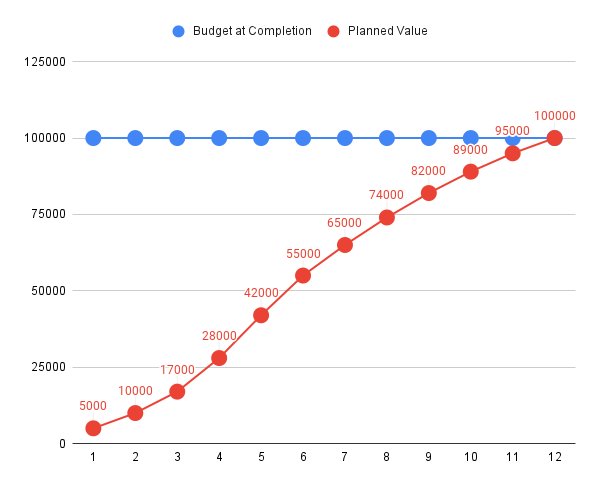
\includegraphics[width=.75\textwidth, keepaspectratio]{img/chart1.png}
    \end{figure}
\end{frame}
\begin{frame}
    \begin{figure}[htp]
        \centering
        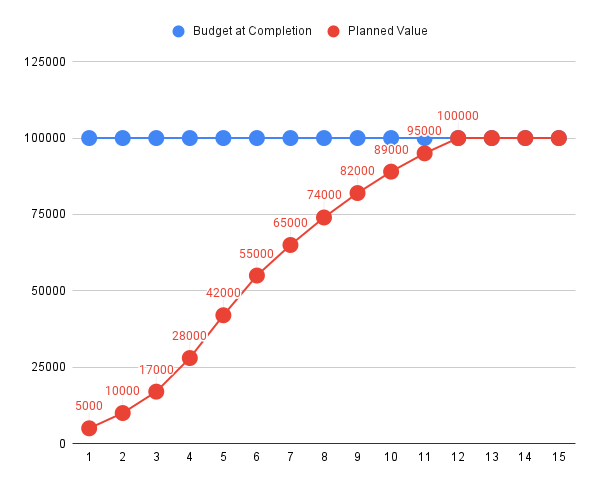
\includegraphics[width=.75\textwidth, keepaspectratio]{img/chart2.png}
    \end{figure}
\end{frame}
\begin{frame}[fragile]
    \frametitle{Berechnung der Effizienz}
    \LARGE
    \begin{itemize}
        \item (CPI) Cost Performance Index
        \begin{center}
            CPI = EV / AC
        \end{center}
        \item[]
        \item (SPI) Schedule Performance Index
        \begin{center}
            SPI = EV / PV
        \end{center}
    \end{itemize}
\end{frame}
\begin{frame}[fragile]
    \huge
    Frage - Inwieweit oder wie genau kann der Grad entschieden werden?
\end{frame}


\section{Prognosen}
\begin{frame}[fragile]
    \frametitle{Gesamtkostenprognose}
    \Large
    Mit Hilfe der berechneten Werte können Prognosen für den weiteren Projektverlauf erstellt werden
    Hier als Beispiel monetare Kosten zum Projektende
    \begin{itemize}
        \item Verschiedene Rechnungsmethode denkbar
    \end{itemize}
    Daumenregel: Überschrittenes Budget kann tendenziell nicht wieder ausgeglichen werden
    \begin{itemize}
        \item Kosten werden meist minimal abgeschätzt
    \end{itemize}
\end{frame}
\begin{frame}[fragile]
    \frametitle{Gesamtkostenprognose}
    \Large
    Annahme 1: Der Rest des Projektes verläuft wie \textbf{geplant}
    \begin{itemize}
        \item AC + noch geplanten Ausgaben
    \end{itemize}
    \bigbreak
    Annahme 2: Der Rest des Projektes verläuft wie \textbf{bisher}
    \begin{itemize}
        \item AC + (noch geplanten Kosten * CPI)
    \end{itemize}
    \bigbreak
    Annahme 3: Durchschnitt der beiden bisherigen Prognosen
    \begin{itemize}
        \item (Prognose1 + Prognose2) / 2
    \end{itemize}
\end{frame}


\section{Verbesserungen}
\begin{frame}[fragile]
    \frametitle{Einführung der Earned Schedule}
    \begin{center}
        \LARGE
        SPI = EV / PV
    \end{center}
\end{frame}
\begin{frame}[fragile]
    \frametitle{Einführung der Earned Schedule}
    \begin{center}
        \LARGE
        SPI = EV / PV
    \end{center}
    \Large
    \begin{itemize}
        \item SPI nur bedingt aussagekräftig
        \item Gegen Ende des Projektes läuft SPI gegen 1
        \begin{itemize}
            \item Gegen Ende des Projektes sollte \textbf{EV = EAC} sein
            \item EV läuft unaufhaltbar gegen EAC
            \item PV läuft unaufhaltbar gegen EAC
        \end{itemize}
        \item Informationen wie "zu spät" oder "früher als geplant" gehen verloren
    \end{itemize}
\end{frame}


\section{Software Development}
\begin{frame}[fragile]
    Was muss getan werden um "earned value" auf Softwareentwicklung anzuwenden?
    \begin{itemize}
        \item Wochen als Iterationen interpretieren
        \item Kosten der Arbeitspakete aufsummieren
    \end{itemize}
\end{frame}
\begin{frame}[fragile]
    Problem - Arbeitspakete sind meist parallel
    \begin{itemize}
        \item Wie gut kann die Methode damit umgehen?
        \item Inwieweit sind Pakete halb fertig?
    \end{itemize}
\end{frame}


\end{document}
